\chapter{Result and conclusion}
Choosing a wrong strategy to parallelize a given function is critical error in an OpenCL implementation. Parallelism, while being advantageous to the performance, requires a lot of thought of what to parallelize, and how to utilize the full potential of parallelism for a given task. In the last chapters, an implementation for shifting algorithm was presented as well as in-depth discussions about the strategy, the optimization, and the possible errors in the process. With the gained knowledge, a further improvement was gained for the development of the robot and opens up new possibilities in another computation areas.

The result is roughly 4x better than a traditional, with processor implementation. Average execution time and concrete result data from 10 test probes for each resolution are presented as following, regarding the example point clouds and devices, for both systems in test, first with AMD RX460:

\begin{figure}[H]
	\centering
	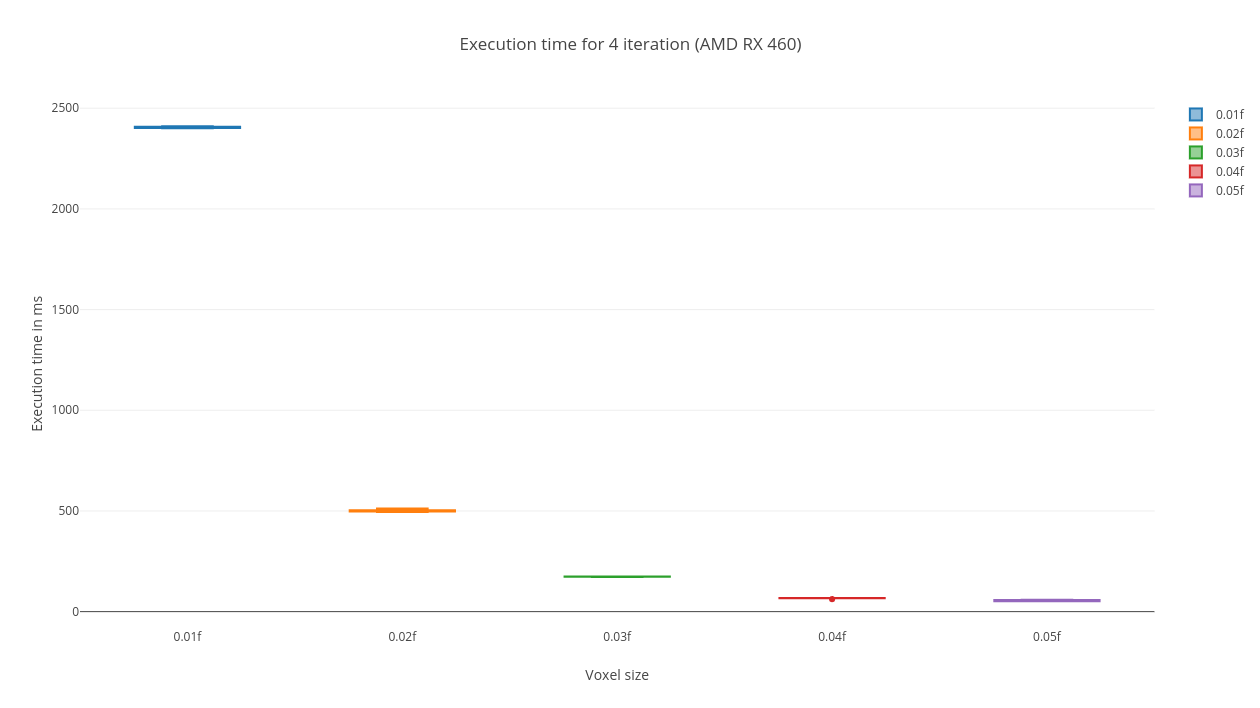
\includegraphics[width=14cm]{images/AllfouriterationRX460.png}
	\caption{Execution time for 4 iterations with AMD RX460}
	\label{ExampleOCTImage}
\end{figure}
\pagebreak

\begin{table}[H]
\centering
\caption{Concrete Execution time (AMD RX 460)}
\begin{tabular}{llllll}
   & 0.01f & 0.02f & 0.03f & 0.04f & 0.05f \\
1  & 2408  & 497   & 174   & 62    & 55    \\
2  & 2406  & 503   & 172   & 67    & 52    \\
3  & 2409  & 499   & 173   & 68    & 39    \\
4  & 2407  & 499   & 174   & 68    & 58    \\
5  & 2400  & 503   & 174   & 67    & 59    \\
6  & 2410  & 498   & 172   & 67    & 52    \\
7  & 2406  & 511   & 174   & 68    & 58    \\
8  & 2402  & 497   & 173   & 67    & 52    \\
9  & 2402  & 512   & 174   & 67    & 51    \\
10 & 2406  & 495   & 174   & 68    & 58   
\end{tabular}
\end{table}
And with the second setup, NVIDIA TITAN X:

\begin{figure}[H]
	\centering
	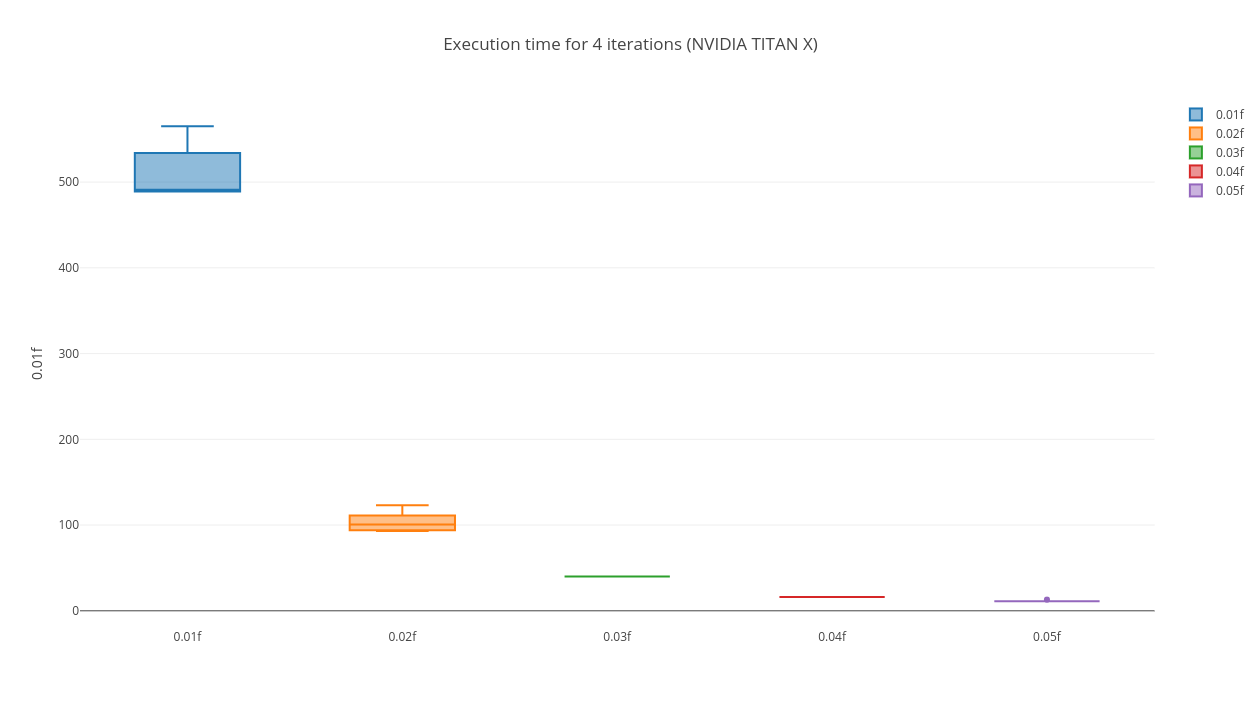
\includegraphics[width=14cm]{images/AllfourIterationTITANX.png}
	\caption{Execution time for 4 iterations with NVIDIA TITAN X}
	\label{ExampleOCTImage}
\end{figure}

\begin{table}[H]
\centering
\caption{Concrete Execution time (NVIDIA TITAN X)}
\begin{tabular}{llllll}
   & 0.01f & 0.02f & 0.03f & 0.04f & 0.05f \\
1  & 557   & 123   & 40    & 16    & 13    \\
2  & 565   & 111   & 40    & 16    & 11    \\
3  & 489   & 100   & 40    & 16    & 11    \\
4  & 489   & 120   & 40    & 16    & 11    \\
5  & 490   & 111   & 40    & 16    & 11    \\
6  & 489   & 101   & 40    & 16    & 11    \\
7  & 491   & 93    & 40    & 16    & 11    \\
8  & 491   & 93    & 40    & 16    & 11    \\
9  & 492   & 94    & 40    & 16    & 11    \\
10 & 534   & 94    & 40    & 16    & 11   
\end{tabular}
\end{table}

In the two illustrations the vertical axis stands for the execution time for all iterations in milliseconds and the horizontal axis stands for resolution of the point clouds. The size of points in source and model point clouds directly depend on the solution, with concrete numbers presented as following :



\begin{table}[H]
\centering
\caption{Point cloud sizes with corresponding resolution}
\label{my-label}
\begin{tabular}{llllll}
Resolution         & 0.01f & 0.02f & 0.03f & 0.04f & 0.05f \\
Source Point cloud & 9037  & 2289  & 1159  & 557   & 462   \\
Model Point Cloud  & 2037  & 1225  & 716   & 428   & 283  
\end{tabular}
\end{table}
\newpage
The results show a notable correlation between the resolution and execution time :  The bigger the size of model and source point clouds, the slower the execution. A dramatic change could be seen between 0.02f and 0.01f, when the size of source point cloud quadruples its size and the model has almost two times more points. These difference in model size heavily changes the time needed to reserve memory and execute kernels. However, a closer investigation in execution time in these steps shows a different changes between them : bigger sized model and source point cloud slow down the second step (finding correspondence) drastically, whereas does not have much effect on to first (transforming point cloud) and third step (sum up result). The difference lies between the tasks of those kernels : While first and third step are independent from the point cloud sizes, the second step is about looping through the source point cloud to find correspondence, which consequently would take longer for bigger point cloud. 

For the resolution used in the example, which is 0.02f, the performance of each step mentioned in the last chapter, is presented in the following figures, start with the AMD setup:

\begin{figure}[H]
	\centering
	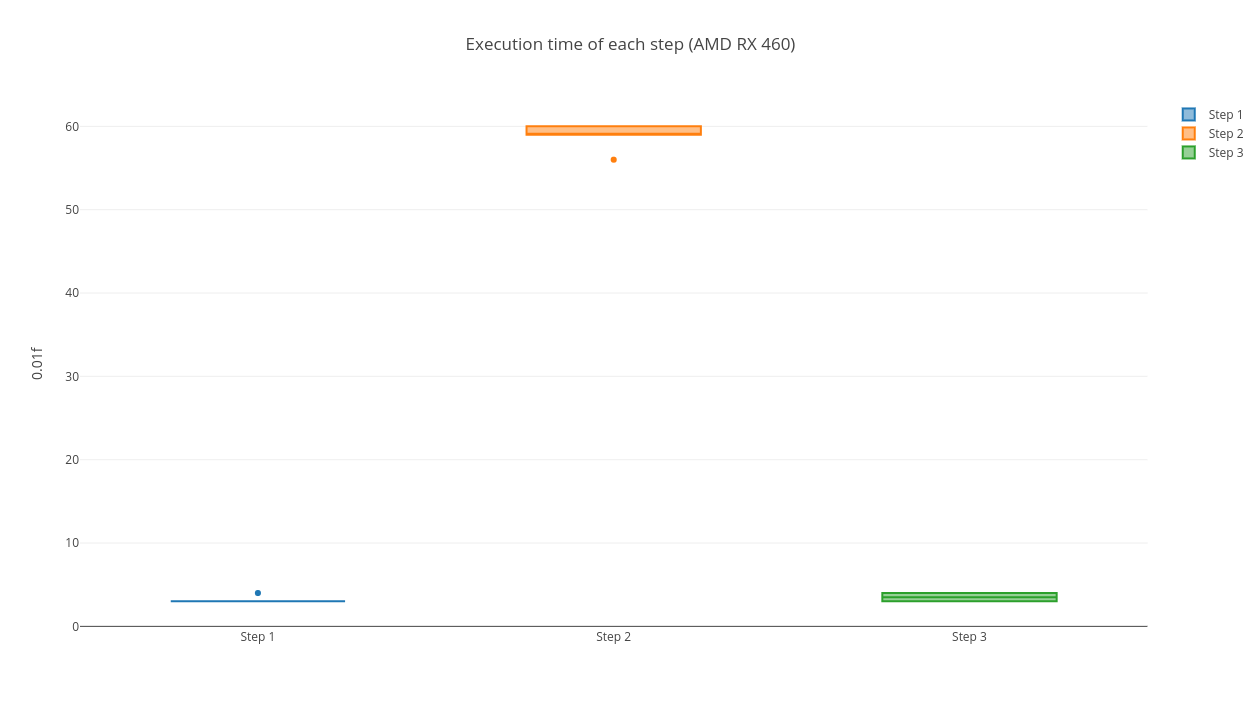
\includegraphics[width=14cm]{images/EachstepAMD.png}
	\caption{Execution time for each step with AMD RX460}
	\label{ExampleOCTImage}
\end{figure}

\newpage
\begin{table}[H]
\centering
\caption{Concrete Execution time for each step (AMD RX 460)}
\begin{tabular}{llll}
   & Step 1 & Step 2 & Step 3 \\
1  & 3      & 59     & 3      \\
2  & 3      & 59     & 4      \\
3  & 3      & 59     & 4      \\
4  & 4      & 60     & 3      \\
5  & 3      & 59     & 4      \\
6  & 3      & 59     & 3      \\
7  & 3      & 59     & 4      \\
8  & 3      & 56     & 3      \\
9  & 3      & 59     & 4      \\
10 & 3      & 60     & 3     
\end{tabular}
\end{table}
And for NVIDIA setup:

\begin{figure}[H]
	\centering
	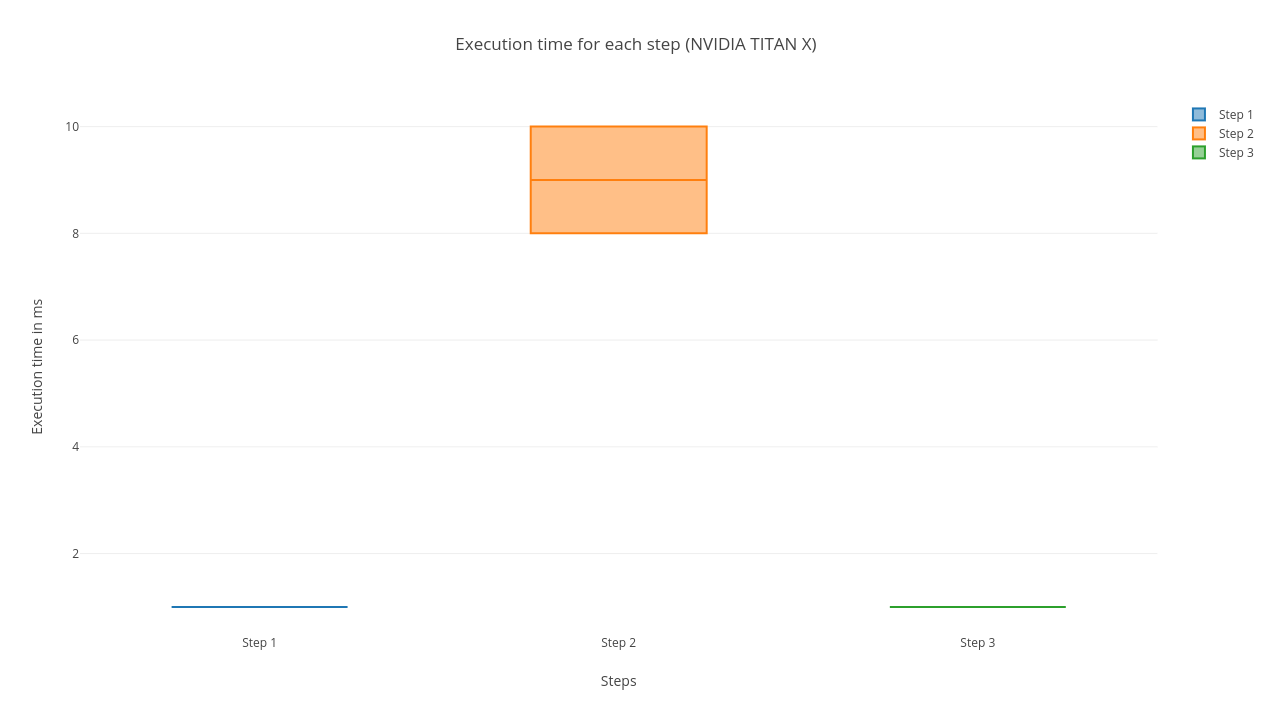
\includegraphics[width=14cm]{images/EachStepNVIDIA.png}
	\caption{Execution time for each step with NVIDIA TITAN X}
	\label{ExampleOCTImage}
\end{figure}
\begin{table}[H]
\caption{Concrete Execution time for each step (NVIDIA TITAN X)}
\centering
\begin{tabular}{llll}
   & Step 1 & Step 2 & Step 3 \\
1  & 1      & 10     & 1      \\
2  & 1      & 10     & 1      \\
3  & 1      & 9      & 1      \\
4  & 1      & 8      & 1      \\
5  & 1      & 8      & 1      \\
6  & 1      & 10     & 1      \\
7  & 1      & 9      & 1      \\
8  & 1      & 8      & 1      \\
9  & 1      & 8      & 1      \\
10 & 1      & 10     & 1     
\end{tabular}
\end{table}
A significant improvement in performance in step 2 shows how computational resource demanding the kernel function is. It often takes up to 90\% of total performance time and shows the best improvements with better hardware. The execution time in this step depends solely and heavily on the clock speed of each processing unit and access speed to the global memory of the physical device.

In conclusion, the OpenCL Implementation shows a better performance than the CPU implementation. It is roughly 15-20x times faster for the NVIDIA setup and 4-5x times faster for a AMD setup, with both of these devices available for off the shelf purchase. It also opens up the possibility of using more than GPU devices and reduce the workload of the CPU. The end performance is far more reliable and is a step forward in development of the robotic system. 

The possibility of a better result does not stop there, since the GPU still has not used all available computing power. A potentially better strategy to parallelize the task by using more work units might result into a much better execution time, or a different approach can be applied in the second step, the most time consuming part of the algorithm. However, within the scope of this thesis, another approach will not be investigated and leaves room for improvement in further development. 


